\chapter{Grundlagen}\label{basics}
Zunächst wird für diese Arbeit ein geeignetes Speicherformat für 3D Modelle von Gebäuden benötigt.
Um den Bau von Gebäuden zu automatisieren, ist es notwendig die Domäne \textit{Gebäude} möglichst vollständig digital abbilden zu können. 
Hilfreich ist dabei, wichtige Daten über bestimmte Bestandteile des Gebäudes direkt in das Modell zu integrieren, auf Basis derer etwa Kostenberechnungen durchgeführt oder Materialmengen abgeschätzt werden können.
Da diese Informationen oft von Experten verschiedener Fachbereiche (etwa aus den Bereichen der Architektur, des Bauwesens oder der Statik) stammen, muss das Format flexibel und im besten Fall auch zeitgleich bearbeitbar sein.
Dafür werden seit dem Jahr 2000 die \textit{Industry Foundation Classes} (IFC) von buildingsmart entwickelt, deren Anwendung im internationalen Bauwesen mittlerweile weit verbreitet ist~\cite{Industry61:online}.


\section{Industry Foundation Classes}\label{basics:ifc}
In der Spezifikation des Standards selbst, wird dieser wie folgt beschrieben (aus dem Englischen):
\glqq{}Die Industry Foundation Classes (IFC) sind ein offener internationaler Standard für Daten des Building Information Model (BIM), welche zwischen Softwareanwendungen ausgetauscht, gemeinsam genutzt und von den verschiedenen Akteuren der Bauindustrie und des Gebäudemanagements verwendet werden. 
Der Standard enthält Definitionen für Daten, die für die Lebenszyklen von Gebäude- und Infrastrukturarbeiten erforderlich sind. 
Die bis jetzt in die IFC aufgenommenen Infrastruktur-Typen umfassen Brücken, Straßen, Eisenbahnen, Wasserstraßen und Hafenanlagen\grqq{}~\cite{IFCScope:online}. 
Eine frühere Version des IFC Standards ist unter der Bezeichnung ISO 16739 registriert (siehe~\cite{ISOISO1694:online}).
Da der IFC aber nach wie vor kontinuierlich weiterentwickelt wird, wird in dieser Arbeit die derzeit neueste Version verwendet.
Diese ist die IFC Spezifikation 4.3.1.0~\cite{IFC4310Spezification:online}.
Das verbreitetste Austauschformat für IFC ist das \textit{Step Physical File Format}, welches im ISO 10303 Teil 21 registriert ist~\cite{ISO_Step:online}.
Zudem gibt es speicherreduzierte Formate wie ifcZip oder für Menschen lesbare Formate wie ifcXML~\cite{Industry93:online}\cite{IFCForma28:online}\cite{BIM_handbook_AEC_XML_SCHEMAS}.

\subsection{IFC 4.3.1.0 Aufbau}
Im Grunde definieren die \textit{Industry Foundation Classes} eine Vielzahl an Klassen, die in einer komplexen Hierarchie angeordnet den Grundstock des Datenmodells bilden.
Diese sind anfangs abstrakte Konzepte, die sich mit zunehmender Tiefe in der Hierarchie konkretisieren.
\begin{figure}[ht]
    \centering
    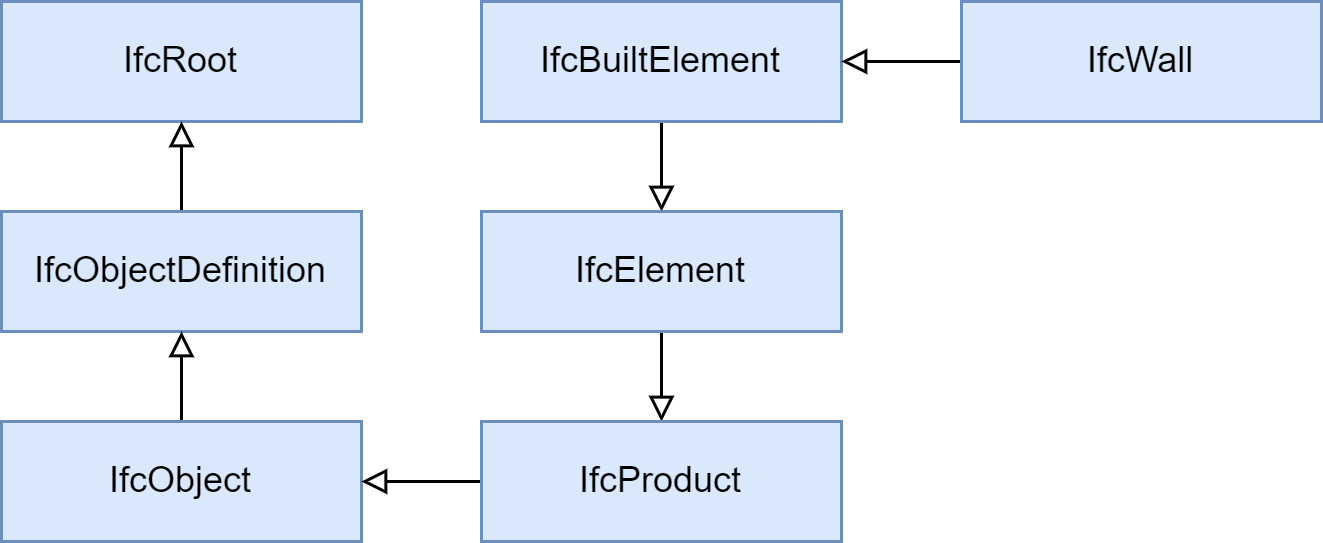
\includegraphics[width=0.6\columnwidth]{fig/Hierarchie_IfcWall_300.drawio.png}
    \caption{Klassenhierarchie am Beispiel der Klasse \textit{IfcWall}.}\label{fig:IfcWall_Hierarchie}
\end{figure}
Da sich diese Arbeit zum größten Teil mit aus Wänden bestehenden Gebäuden befasst, wird nachfolgend die Klasse \textit{IfcWall} wiederholt als Beispiel herangezogen.
Der für diese Klasse relevante Ausschnitt aus der Klassenhierarchie ist in Abbildung~\ref{fig:IfcWall_Hierarchie} dargestellt.
Objekte werden von dem Standard in Relation zueinander gestellt, um komplexere Zusammenhänge darzustellen.
In Abbildung~\ref{fig:IFC_Relationships} erkennt man den Zusammenhang zwischen einem Objekt des Typs \textit{IfcWall}, des Stockwerks, welches diese Wand referenziert und wiederum selbst Teil eines \textit{IfcBuildings} ist, bis hin zur obersten Komponente eines IFC Projektes, dem gleichnamigen \textit{IfcProject}.

\begin{figure}[h]
    \centering
    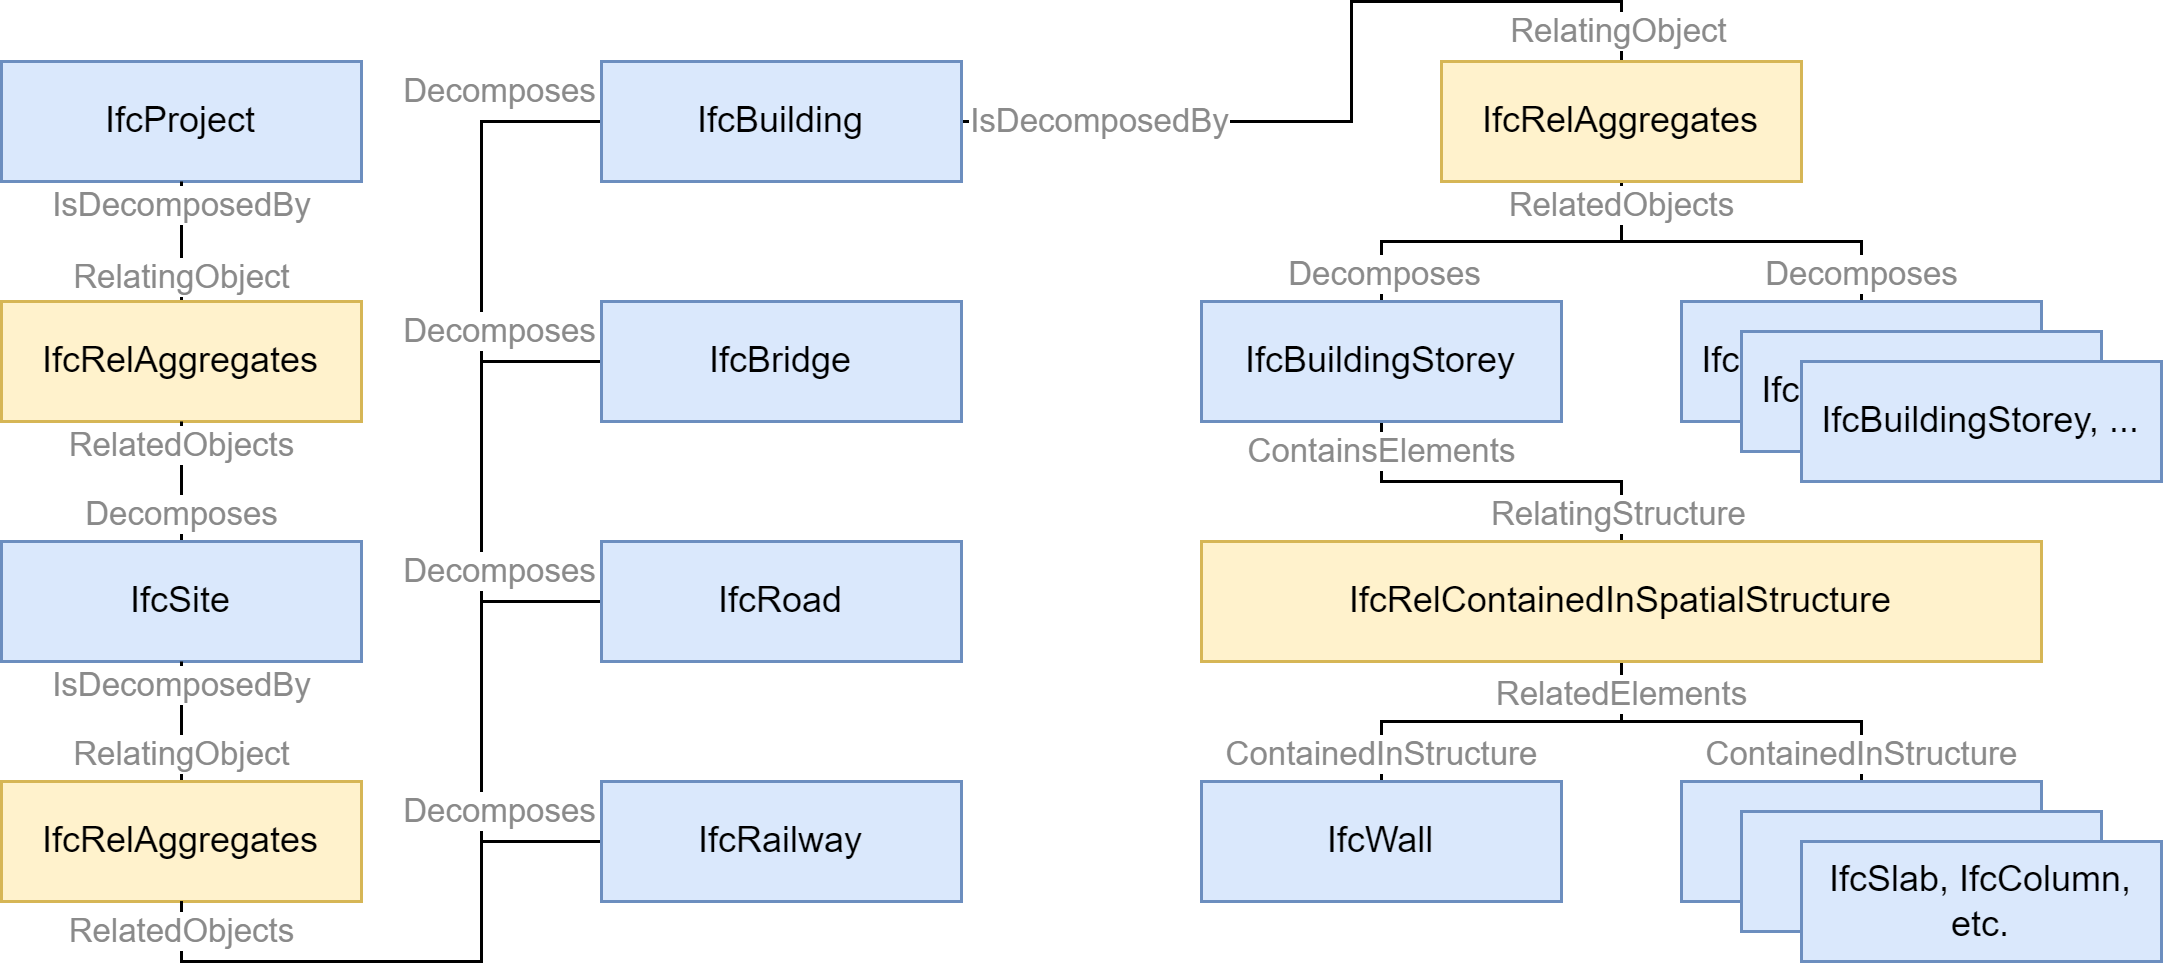
\includegraphics[width=0.9\columnwidth]{fig/IFC_Relationships_300.drawio.png}
    \caption{Relation der IfcWall und einem \textit{IfcProject}.}\label{fig:IFC_Relationships}
\end{figure}

\subsection{IfcPropertySets und IfcQuantitySets}\label{basics:ifc_properties}
Mit dem Erweitern des Gebäudemodells um möglichst viele Informationen, schafft man einen detaillierten digitalen Zwilling, der neben der bloßen Darstellung des Gebäudes als 3D Modell zusätzlich die Untersuchung auf andere Eigenschaften ermöglicht.
Dazu zählen zum Beispiel eine präzisere Kosten- und Zeitschätzung, Sicherheitsaspekte und Emissionen eines Bauvorhabens~\cite{Industry93:online}~\cite{Ding2014}. 
Dies ist mithilfe von \textit{IfcPropertySets} und \textit{IfcQuantitySets} umsetzbar, welche Objekten oder Objekttypen angehängt werden können.
Dabei werden IfcQuantitySets vorwiegend dazu verwendet numerische Werte zu geometrischen oder physikalischen Eigenschaften auszudrücken.
IfcPropertySets dienen hingegen dazu bestimmten Objekten oder Objekttypen mit sämtlichen nicht numerischen Werten zu annotieren.
Beispiele dafür sind etwa Material oder Farbe eines bestimmten Objekts.
Die Verwendung der Bezeichnung \textit{Set} rührt daher, dass diese Informationen in einer Baumstruktur vorliegen und demnach verschachtelt sein können.
Es gibt zu vielen Klassenbeschreibungen des IFC Standards vordefinierte IfcPropertySetTemplates.
Das hilft dabei wichtige Informationen zu bestimmten Objekttypen einheitlich angeben zu können.
Im Falle des \textit{IfcWallType} existiert beispielsweise das IfcPropertySet mit dem Namen \textit{Pset\_WallCommon}~\cite{IFC4310PSetWallCommon:online}.
Darin können die Ersteller von neuen WallTypes unter anderem Informationen über Brennbarkeit, thermisches Verhalten oder Akustik hinterlegen.
Bei Erzeugung einer IfcWall Instanz aus einem bestimmten WallType sind die damit verbundenen Property- und QuantitySets automatisch damit verknüpft, sodass jedes Objekt relevante Informationen über sich selbst bereithält.
Dies ermöglicht eine effiziente Inspektion des Gebäudemodells.

\subsection{Positionierung von \textit{IfcProducts}}
Die Platzierung eines \textit{IfcProducts} wird durch eine Verkettung relativer Transformationen ausgehend vom \textit{IfcProduct}, über sämtliche Strukturen, die dieses Objekt enthalten, bis hin zur \textit{IfcSite} realisiert~\cite{IFCPlatzierung}.
Diese Hierarchie kann der Abbildung~\ref{fig:IFC_Relationships} entnommen werden.
Um die globale Position eines \textit{IfcProducts} zu erhalten, müssen die relativen Transformationen miteinander verrechnet werden.
Der IFC Standard unterstützt zudem die Möglichkeit Positionierungen anhand eines Rasters oder mithilfe des sogenannten \textit{linear placements} anzugeben.

\subsection{IfcOpeningElement}\label{basics:IfcOpeningElement}
Neben Wänden stellen Fenster und Türen wichtige Elemente eines Gebäudes dar.
Diese sind ebenfalls Teil der Klassen des IFC Standards.
Objekte des Typs \textit{IfcOpeningElement} dienen dazu, die notwendigen Lücken in einer Wand zu definieren, in die später eine Tür oder ein Fenster eingebaut werden soll.
In der Dokumentation wird dies wie folgt formuliert (aus dem Englischen): \glqq{}[Das IfcOpeningElement] stellt eine Lücke in jedem Element dar, das eine physische Manifestation hat\grqq{}~\cite{IFC4310OpeningElement:online}.
Es gibt zwei Arten der Klasse IfcOpeningElement, je nachdem ob die Öffnung durch die gesamte Breite eines Objektes reicht oder nicht. 
Folglich entsteht dadurch eine Unterscheidung zwischen Nischen und tatsächlichen Öffnungen, wobei nur letztere im Zusammenhang mit Fenstern oder Türen Sinn ergeben.

\section{IFC und Blender}\label{basics:blender}
Blender ist eines der beliebtesten Open-Source-Programme zur Modellierung von 3D Modellen und Animationen~\cite{blendero56:online}.
Eine umfangreiche Python API erlaubt es Blender durch sogenannte Add-ons an die eigenen Bedürfnisse anzupassen~\cite{PythonWebsite:online}~\cite{BlenderPythonAPI:online}.
Aufgrund dessen existiert auch eine Vielzahl an freien Erweiterungen \textendash{} unter anderem auch eine Integration des IFC Standards.

\subsection{blenderbim}\label{basics:blenderbim}
Neben kommerziellen Produkten wie etwa revit von autodesk zur Modellierung von IFC Modellen, gibt es auch für Blender ein freies Plugin, um IFC Modelle zu erstellen~\cite{RevitSof26:online}~\cite{BlenderB43:online}.
Dieses Plugin ermöglicht es neben dem bloßen Designen des Gebäudes in kurzer Zeit zum Beispiel detaillierte Zeichnungen verschiedener Perspektiven herauszuarbeiten, die etwa von Bauingenieuren verwendet werden können, um einzelne Stockwerke oder Verkabelungen zu planen.
Blenderbim selbst kapselt unter anderem die Open Source Python Bibliothek \textit{IfcOpenShell}, sodass diese in der Blender Laufzeitumgebung zur Verfügung steht~\cite{IFCOpenShell:online}.

\subsection{IfcOpenShell}\label{basics:ifcopenshell}
\begin{lstlisting}[label={basics:ifcopenshell_sample_code}, language=Python, caption=Beispielprogramm zur Extraktion bestimmter Daten einer IFC Datei und Generierung eines Meshes aus deren geometrischen Representationen.]
import ifcopenshell
from ifcopenshell import geom
from stl import mesh, Mode
import numpy as np

settings = ifcopenshell.geom.settings()
settings.set(settings.USE_WORLD_COORDS, True)

ifc_file = ifcopenshell.open("model.ifc")
products = ifc_file.by_type("IfcProduct")
meshes = []

for product in products:
    if product.Representation and product.is_a("IfcWall"):
        shape = ifcopenshell.geom.create_shape(settings, product)
        vertices = np.array(shape.geometry.verts).reshape((-1, 3))
        edges = np.array(shape.geometry.edges)
        faces = np.array(shape.geometry.faces).reshape((-1, 3))

        m = mesh.Mesh(np.zeros(faces.shape[0], dtype=mesh.Mesh.dtype))
        for i, f in enumerate(faces):
          for j in range(3):
              m.vectors[i][j] = vertices[f[j], :]
        meshes.append(m)

# Create the combined mesh
combined = mesh.Mesh(np.concatenate([m.data for m in meshes]))
combined.save('model.stl', mode=Mode.ASCII)

\end{lstlisting}

IfcOpenShell ist eine frei verfügbare Bibliothek, die es erleichtert mit Daten im IFC Format zu arbeiten~\cite{IFCOpenShell:online}.
Sie bietet unter anderem eine Python API an und ist wie bereits erwähnt ein Teil des Blender Add-ons blenderbim.
Natürlich ist es dennoch möglich diese Bibliothek auch ohne Blender zu verwenden.
In Listing~\ref{basics:ifcopenshell_sample_code} ist ein Beispielprogramm zu sehen, das aus einer IFC Datei alle Objekte des Typs IfcWall filtert und deren geometrische Repräsentationen in ein herkömmliches Mesh konvertiert.
Auch andere Informationen, wie die in IfcPropertySets enthaltenen Daten, können mit der Bibliothek in ähnlicher Weise extrahiert werden.
Damit existiert ein intuitiver Zugang zu den Daten von IFC Dateien.

\section{Building Information Modeling}\label{basics:bim}
Ein weiterer Punkt, der für die Verwendung von IFC spricht, ist das sogenannte \textit{Building Information Modeling} (BIM)~\cite{Building41:online}.
Ein Definitionsvorschlag lautet wie folgt (aus dem Englischen): \glqq{}BIM ist definiert als der Einsatz von Informations- und Kommunikationstechnologien zur Verschlankung der Prozesse im Lebenszyklus von Gebäuden, um eine sicherere und produktivere Umgebung für die Bewohner zu schaffen, die Umwelt so wenig wie möglich zu belasten und die Effizienz der Betriebsabläufe für die Eigentümer während des gesamten Lebenszyklus des Gebäudes zu erhöhen\grqq{}~\cite{Arayici2010}.
Zum Lebenszyklus eines Gebäudes gehören etwa anfangs das Planen und Designen, später das Bauen, daraufhin das Verwenden und Instandhalten und nach eventuellen Renovierungen das Abreißen.
BIM kommt in all diesen Phasen zum Tragen und erleichtert diese Prozesse durch Anbieten einer einheitlichen Schnittstelle für alle am Infrastrukturbau und -management beteiligten Personen.
Zusätzlich ermöglicht BIM eine exakte Dokumentation des Geschehens in sämtlichen Phasen des Bauwerks, was unter anderem zu einer genaueren Zeit- und Kostenplanung führt~\cite{Ding2014}.
Auch Verantwortlichkeiten sind Teil von BIM, was zu einer erhöhten Produktivität beiträgt.
Um nun das Zusammenarbeiten der unterschiedlichen Fachbereiche zu erleichtern, gibt es sogenannte BIM-Server auf welchen mehrere Personen synchron an einem Projekt arbeiten können.
Dabei können je nach Aufgabenbereich passende Teilansichten des Projektes herangezogen werden.
BIM-Server unterstützen zusätzlich eine Versionierung des Fortschritts an einem Projekt.

In einem Gespräch mit einem Ingenieur aus dem Bereich \glqq{}Energiesystemtechnik\grqq{} kam zur Sprache, dass viele Bereiche von BIM noch keinen Einzug in Deutschland gefunden haben.
Eben jene \glqq{}Kollaboration über einen BIM-Server mit Änderungsmanagement etc.\ [sei] nicht üblich, da noch nicht alle Beteiligten dazu in der Lage sind. Vor allem Bauherren, Architekten und Baufirmen können es nicht\grqq{}.
Weiter sei \glqq{}auch unklar, wer für falsche Angaben haftet und wer die Konsistenz aller Daten gewährleistet\grqq{}.
Auf der anderen Seite sei \glqq{}das im BIM festgelegte Datenformat IFC das Maß der Dinge und auch bei uns so in Verwendung\grqq{}.
Auch das Einpflegen \glqq{}ergänzende[r] Bauteilinformationen (z.B. zu Gewicht, Dämmwert, Recyclebarkeit, \(CO_2\) Fußabdruck, etc.)\grqq{} finden Einsatz und sind Teil seines Alltags.
Für ihn wichtig ist ebenfalls der Betrieb des Gebäudes.
Hier unterstützt BIM, indem sämtliche Teile der Installationen in einem Gebäude, wie zum Beispiel Fensterdichtungen, Kabel, Rohre, Sicherungen oder eine Umwälzpumpe individuelle Teilenummern zugewiesen bekommen, hinter welchen alle Daten wie etwa Hersteller, Bestellnummern, Lebensdauer, Wartungshistorie oder Entsorgungsnachweise vermerkt sind.
Dies wurde allerdings \glqq{}angesichts der Realität der Handwerker und Gebäudenutzer für völlig unrealistisch und auch etwas over-engineered\grqq{} eingestuft.
Trotzdem sei \glqq{}BIM [\ldots] das große Ding in der Bauwelt und der einzige echte Standard\grqq{}.

\section{opensourceBIM}
Während es vorwiegend kommerzielle Produkte gibt, die Unternehmen das Arbeiten mit BIM ermöglichen, existiert auch hier eine aktive Open Source Bewegung.
Unter dem Namen \glqq{}The open source BIM collective\grqq{} oder kurz \glqq{}opensourceBIM\grqq{} werden derzeit um die 70 Repositories betrieben.
Darin enthalten sind unter anderem ein BIM-Server inklusive verschiedener Clients für Endanwender auf unterschiedlichen Systemen und Werkzeuge, die es erleichtern den IFC Files zu arbeiten~\cite{Theopens96:online}.
Ein kurzer Test hat gezeigt, dass die in Blender modellierte IFC Files tatsächlich über einen \glqq{}Anzeige-Client\grqq{}, der mit einem lokal gehosteten BIM-Server verbunden ist, dargestellt und inspiziert werden können.
Obwohl die Verwendung des BIM-Servers für diese Arbeit nicht notwendig ist, besteht die Option diesen künftig mit in den Workflow zu integrieren, da damit auch das simultane Arbeiten an einem IFC File möglich ist, was in Blender nur teilweise und mit dem Einsatz von Plugins ermöglicht wird.
Das stellt einen Praxisbezug zum aktuell verwendeten Stand dieser Technologien her, was in der oftmals konzeptionellen Natur der Forschung nicht immer der Fall ist.
Wie auch Blender unterstützt BIM-Server das Einbinden von eigenen Plugins, sodass eine Erweiterung um neue Funktionalität möglich ist.
Die Plugins werden in Java geschrieben.
Der Server bietet aber auch eine REST Schnittstelle an, um Clients in anderen Sprachen anzubinden.

\section{Mauerwerksbau}\label{basics:Mauerwerksbau}
Der Mauerwerksbau ist eine Art des Massivbaus, bei welchem Natur- oder Formsteine aufgeschichtet werden, um Wände beziehungsweise Mauern zu errichten.
Eine derart erbaute Wand besteht demnach aus (Bau)-Steinen und den dazwischen entstehenden Fugen.
Mörtel ist dabei nicht zwangsläufig notwendig.
\begin{figure}[hb]
  \centering
  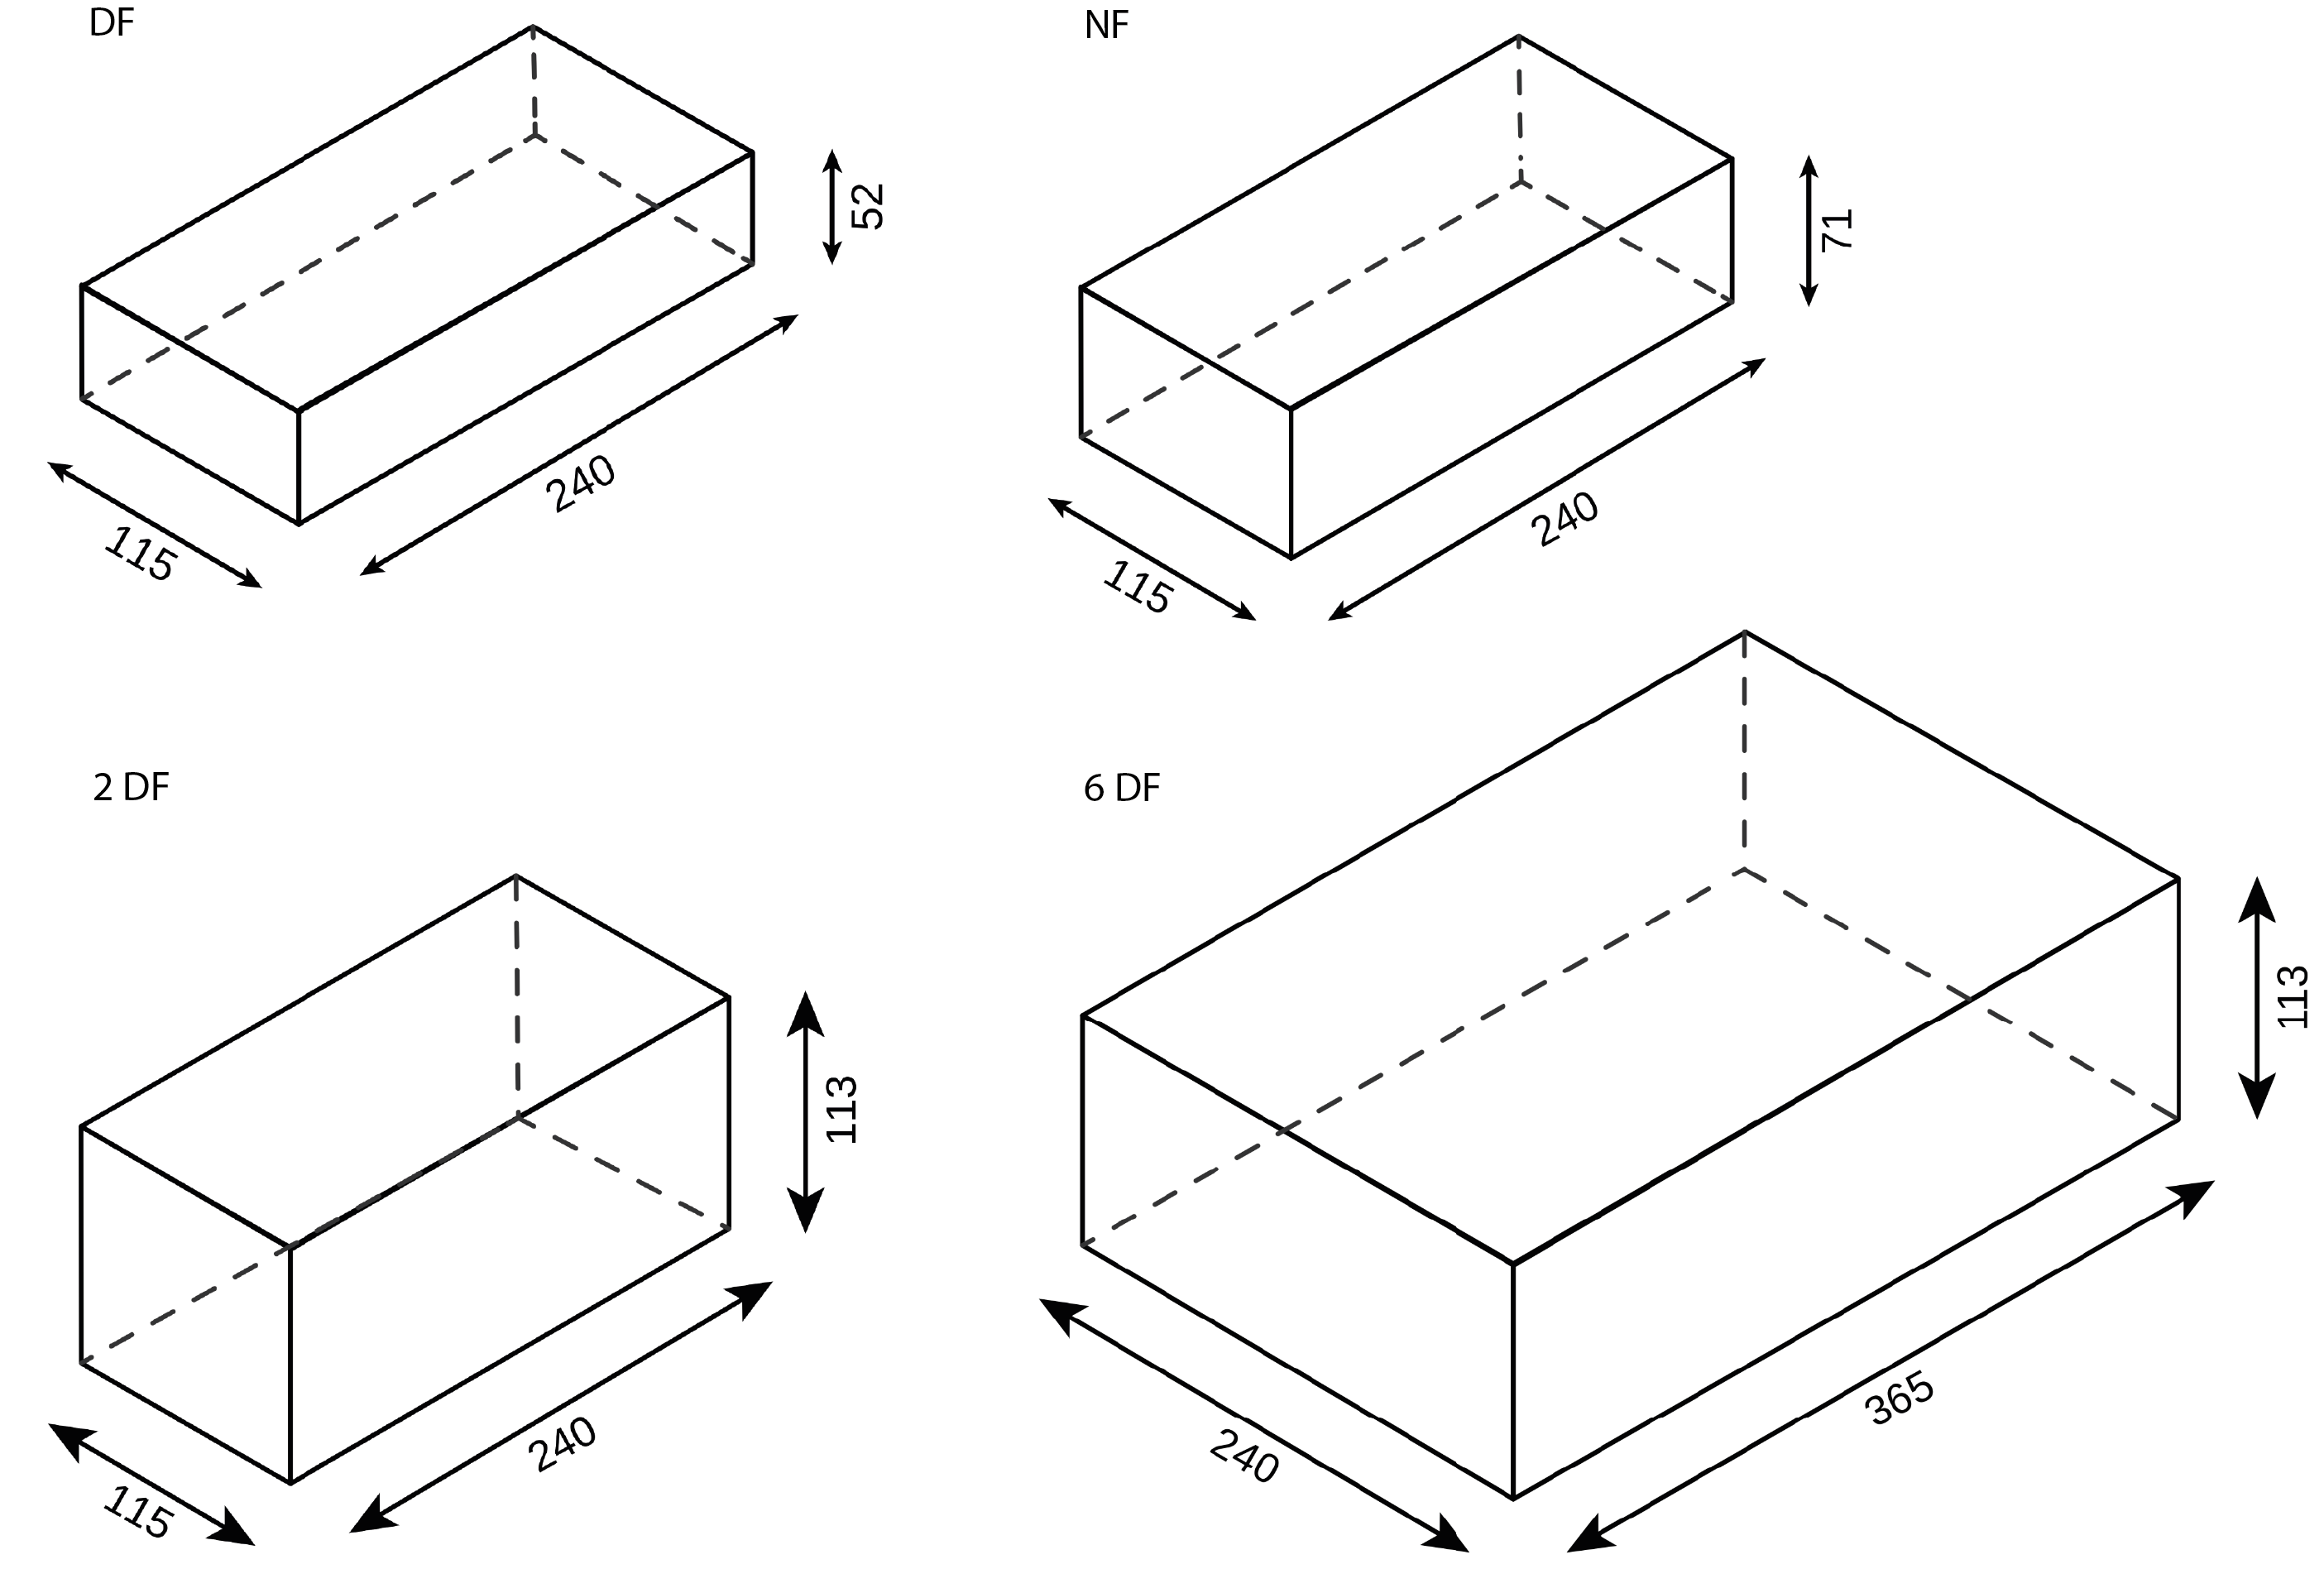
\includegraphics[width=0.7\columnwidth]{fig/Ziegelsteinformate DF NF 2DF 6DF.png}
  \caption{Darstellung verschiedener Steinformate nach DIN 4172 (Baunennmaß in Millimetern)~\cite{Steinfor38:online}}\label{fig:basics:Steinformate}
\end{figure}
Man spricht von trocken versetzten Steinen oder einer Trockenmauer, wenn darauf verzichtet wird.
Heutzutage wird fast ausschließlich mit quaderförmigen Formsteinen gebaut.
Zur Beschreibung solcher Formsteine existieren zwei relevante Größen.
Die eine ist das sogenannte \textit{Baunennmaß}, mit dem die tatsächliche Größe des Steins angegeben wird.
Die andere das \textit{Baurichtmaß}, das sich aus Baunennmaß und dem Fugenmaß zusammensetzt und sozusagen einem Raster entspricht, das durch die Bausteine vorgegeben wird.
\begin{figure}[ht]
  \centering
  \includegraphics[width=0.8\columnwidth]{fig/Oktametrische Maßordnung.png}
  \caption{Besondere Eigenschaften der oktametrischen Maßordnung~\cite{Moro2021}}\label{fig:basics:OktametrischeMassordnung}
\end{figure}

\subsection{Maßsysteme}\label{basics:masssysteme}
Als Maßsystem bezeichnet man die Festlegung der Größen von Bausteinen anhand eines konkret definierten (Grund-) Moduls.
Zwei in Deutschland populäre Grundmodule sind zum einen das \textit{ISO-2848-Basismodul} mit Länge 100 mm und zum anderen der Achtelmeter, verankert in der \textit{DIN 4172 Maßordnung im Hochbau}~\cite{ISO2848}\cite{DIN417224}.
Letzteres bezeichnet man daher auch als das oktametrische Maßsystem.
Nachfolgend wird auf dieses Maßsystem näher eingegangen.

\subsubsection*{Oktametrisches Maßsystem}
Baurichtmaße sind gemäß dem oktametrischen Maßsystem immer ein Vielfaches von \(12.5 cm\) (das entspricht \(1/8 m\)) und nach der Norm aber mindestens \(6.25cm\).
Dies gilt sowohl für Länge und Breite als auch für die Höhe der Steine.
Das System ist in der \textit{DIN 4172 Maßordnung im Hochbau} geregelt und ein fest definiertes Grundmaß für das Bauwesen in Europa~\cite{DIN417224}.
Daraus gehen insbesondere folgende zwei Formate für Ziegelsteine hervor:
das Normalformat (NF) mit \(240\times115\times71 mm\) und das Dünnformat (DF) mit \(240\times115\times52 mm\) (Länge $\times$ Breite $\times$ Höhe)~\cite{Moro2021}.
Alle anderen Formate werden mithilfe dieser beiden Grundsteine angegeben.
So sind zum Beispiel die in Abbildung~\ref{fig:basics:Steinformate} gezeigten 2 DF und 6 DF Steine eine Kombination aus mehreren Steinen im Dünnformat.
Dabei sieht die Norm ein Fugenmaß von \(10 mm\) für Stoßfugen (vertikal) und \(12 mm\) für Lagerfugen (horizontal) vor.
Für Systeme, die eine schmalere oder keine Fuge benötigen, werden entsprechend größere Steine hergestellt, um der Maßordnung weiterhin zu entsprechen.
Durch Einhalten eines Systems ist man zusätzlich in der Lage Türen und Fenster an die daraus entstehenden Öffnungsgrößen anzupassen und vermeidet dadurch zeitaufwendiges, nachträgliches Anpassen oder Spezialanfertigungen.
Da Höhe, Breite und Länge der Steine zusammen mit den dazwischenliegenden Fugen aufgrund des Maßsystems jeweils Vielfache voneinander sind, ergeben sich viele Möglichkeiten zur Aufschichtung und Aneinanderreihung der Bausteine.
Einige davon sind in Abbildung~\ref{fig:basics:OktametrischeMassordnung} zu sehen und sind gleichzeitig Beispiele für einen sogenannten \textit{Mauerwerksverband}.

\begin{figure}[htb]
  \hspace*{\fill}%
  \begin{subfigure}[b]{0.4\columnwidth}
    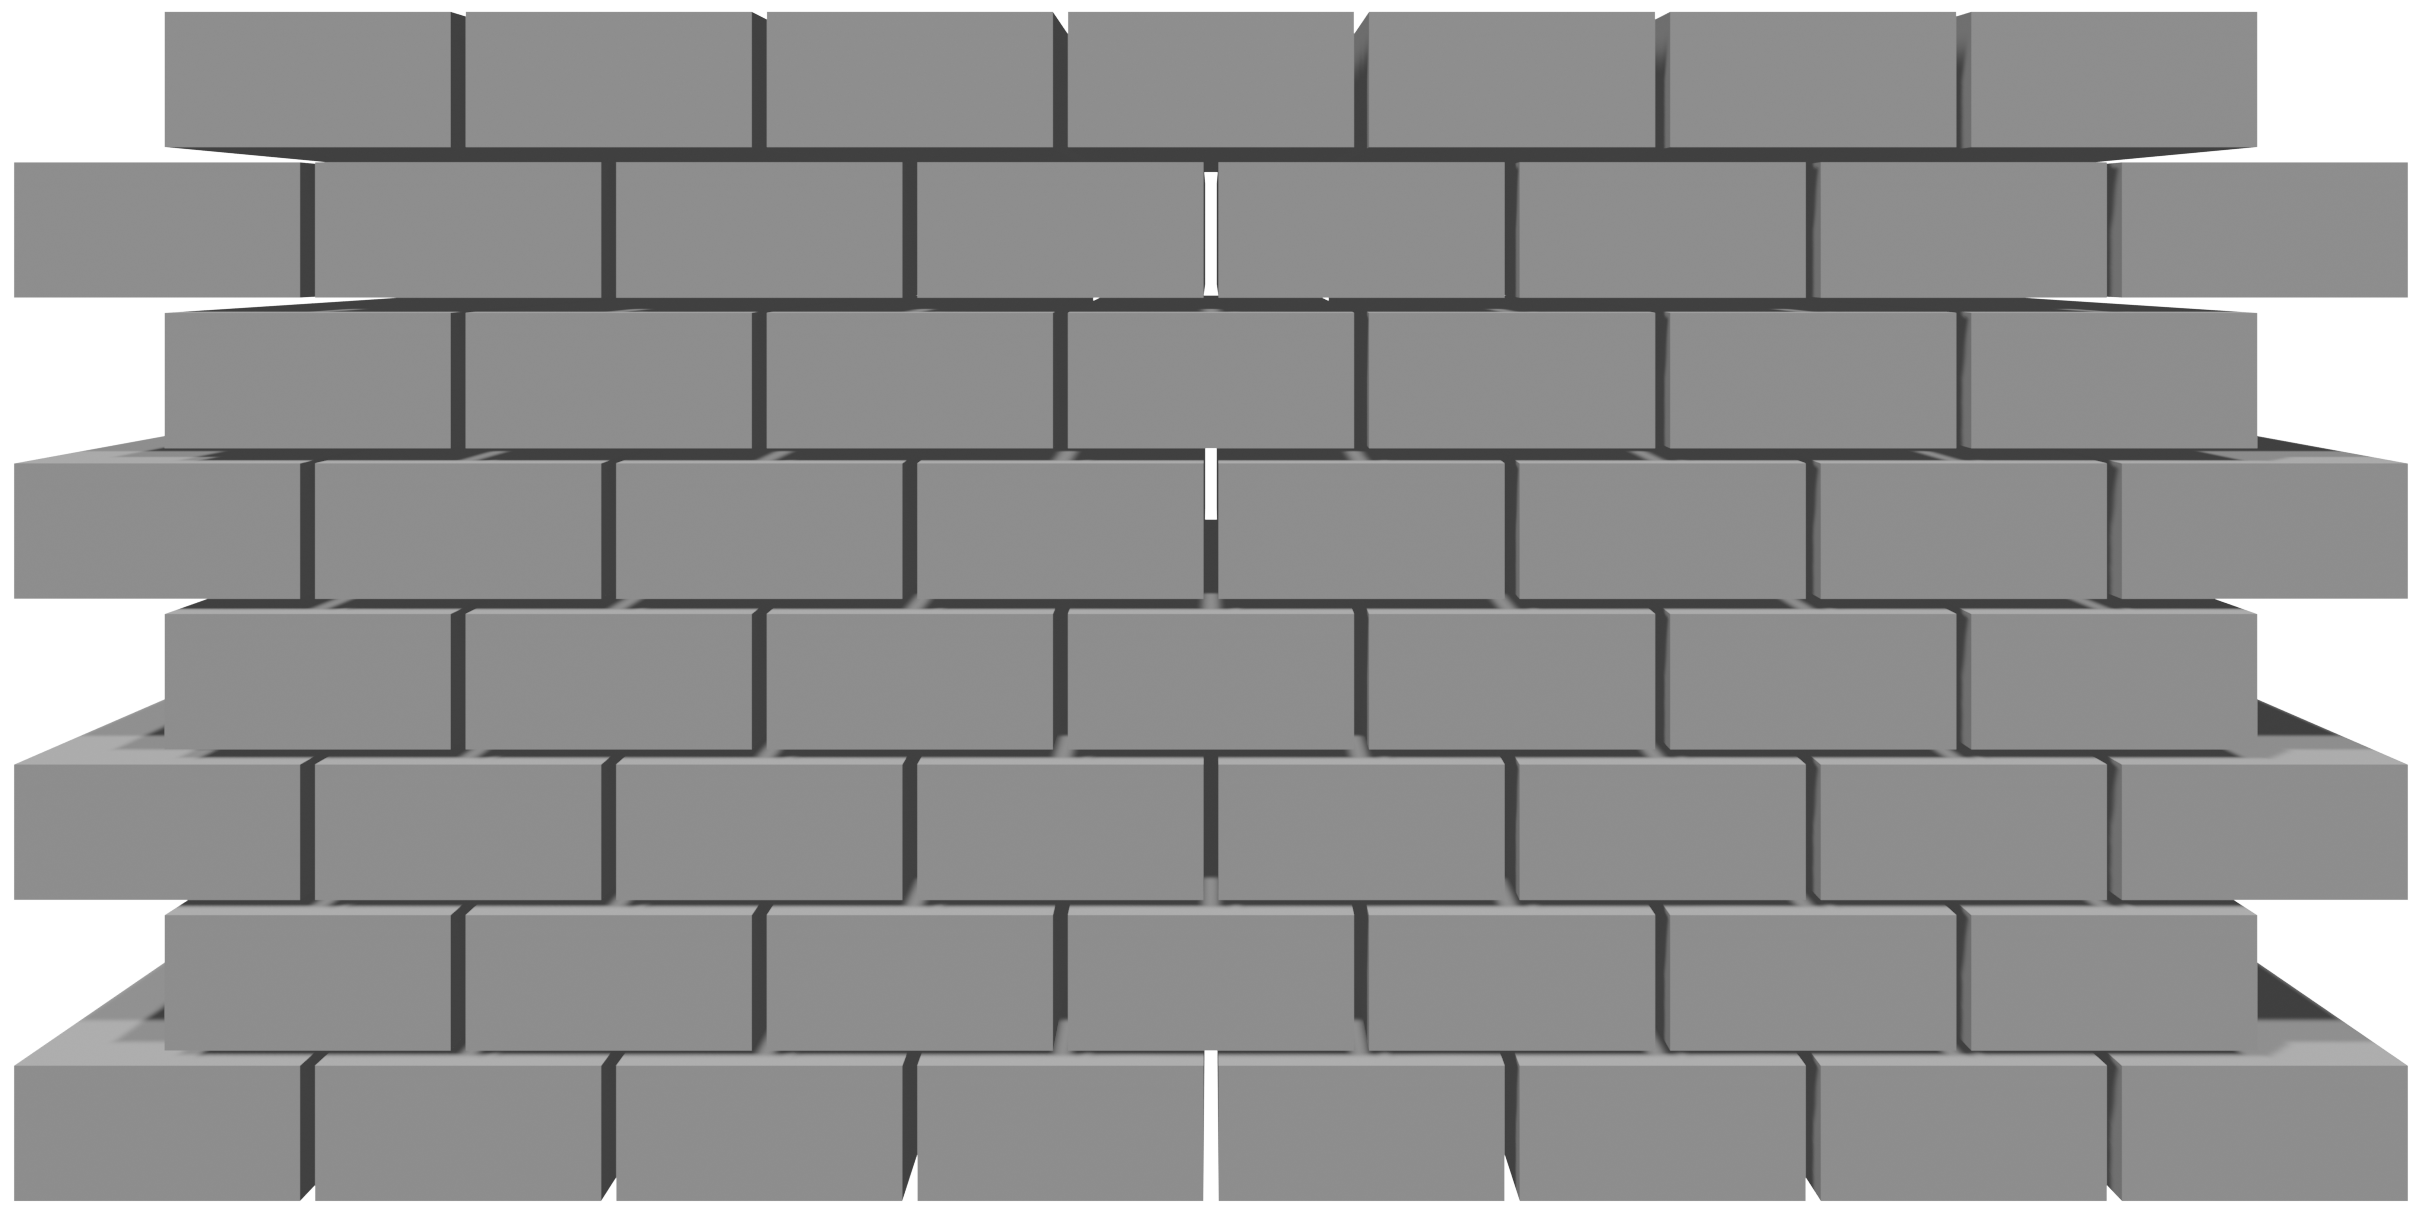
\includegraphics[width=\columnwidth]{fig/basics_headbond.png}
    \caption{Kopfverband.}
  \end{subfigure}
  \hfill
  \begin{subfigure}[b]{0.4\columnwidth}
    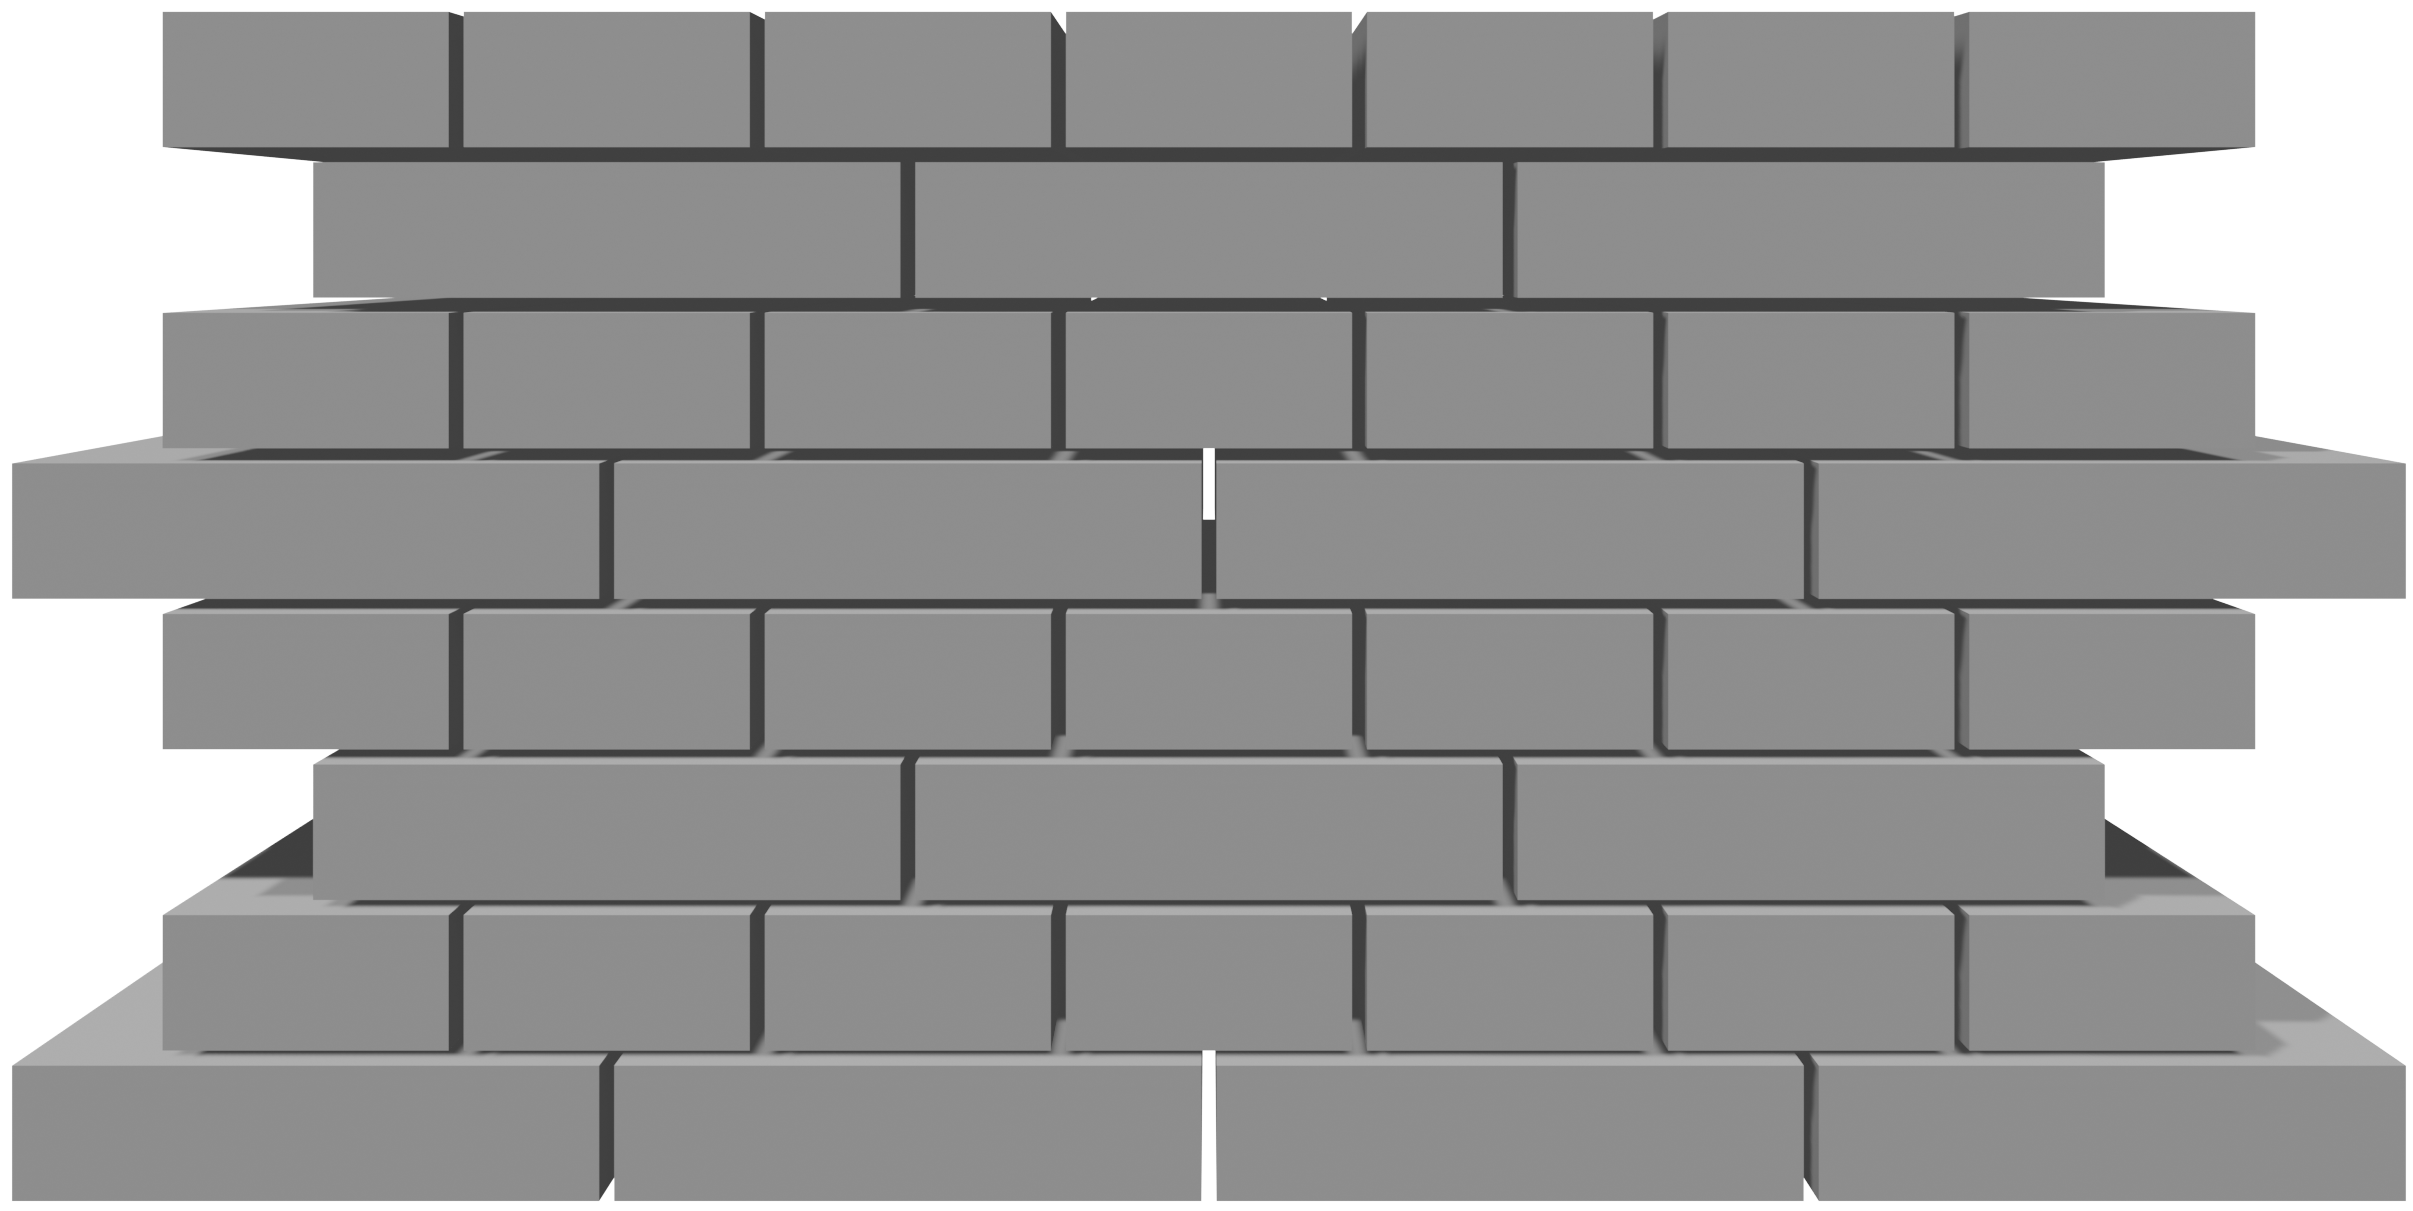
\includegraphics[width=\columnwidth]{fig/basics_crossbond.png}
    \caption{Kreuzverband.}
  \end{subfigure}
  \hspace*{\fill}%
  \begin{subfigure}[b]{0.4\columnwidth}
    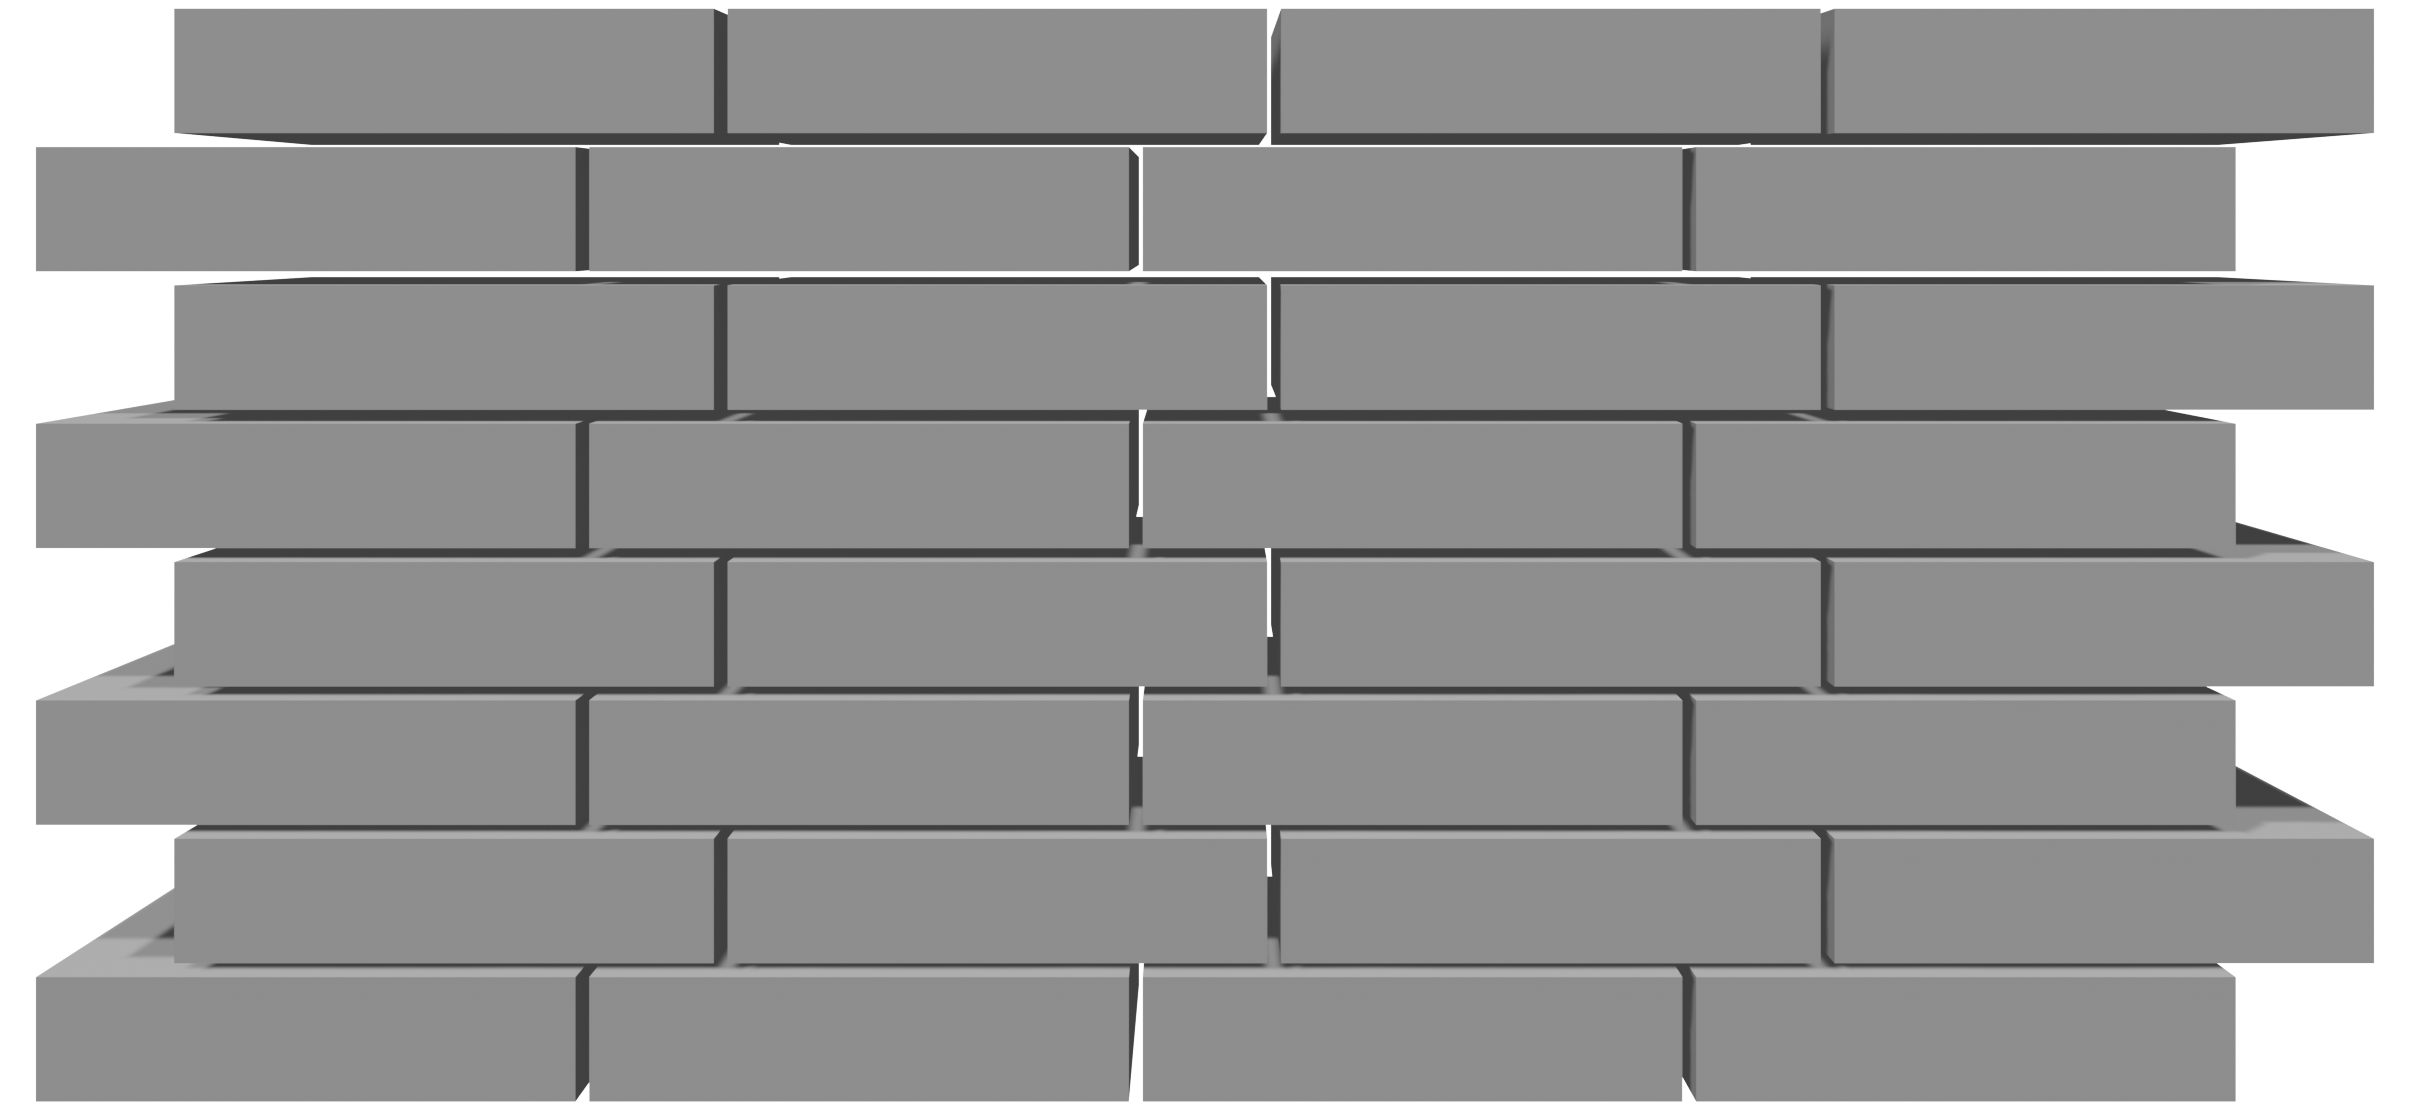
\includegraphics[width=\columnwidth]{fig/basics_stretchedbond25_mittig.png}
    \caption{Mittlerer Läuferverband.}\label{fig:basics:verbaende_c}
  \end{subfigure}
  \hfill
  \begin{subfigure}[b]{0.4\columnwidth}
    
\includegraphics[width=\columnwidth]{fig/basics_stretchedbond25_schleppend}
    \caption{Schleppender Läuferverband.}\label{fig:basics:verbaende_d}
  \end{subfigure}
  \hspace*{\fill}%
  \begin{subfigure}[b]{0.4\columnwidth}
    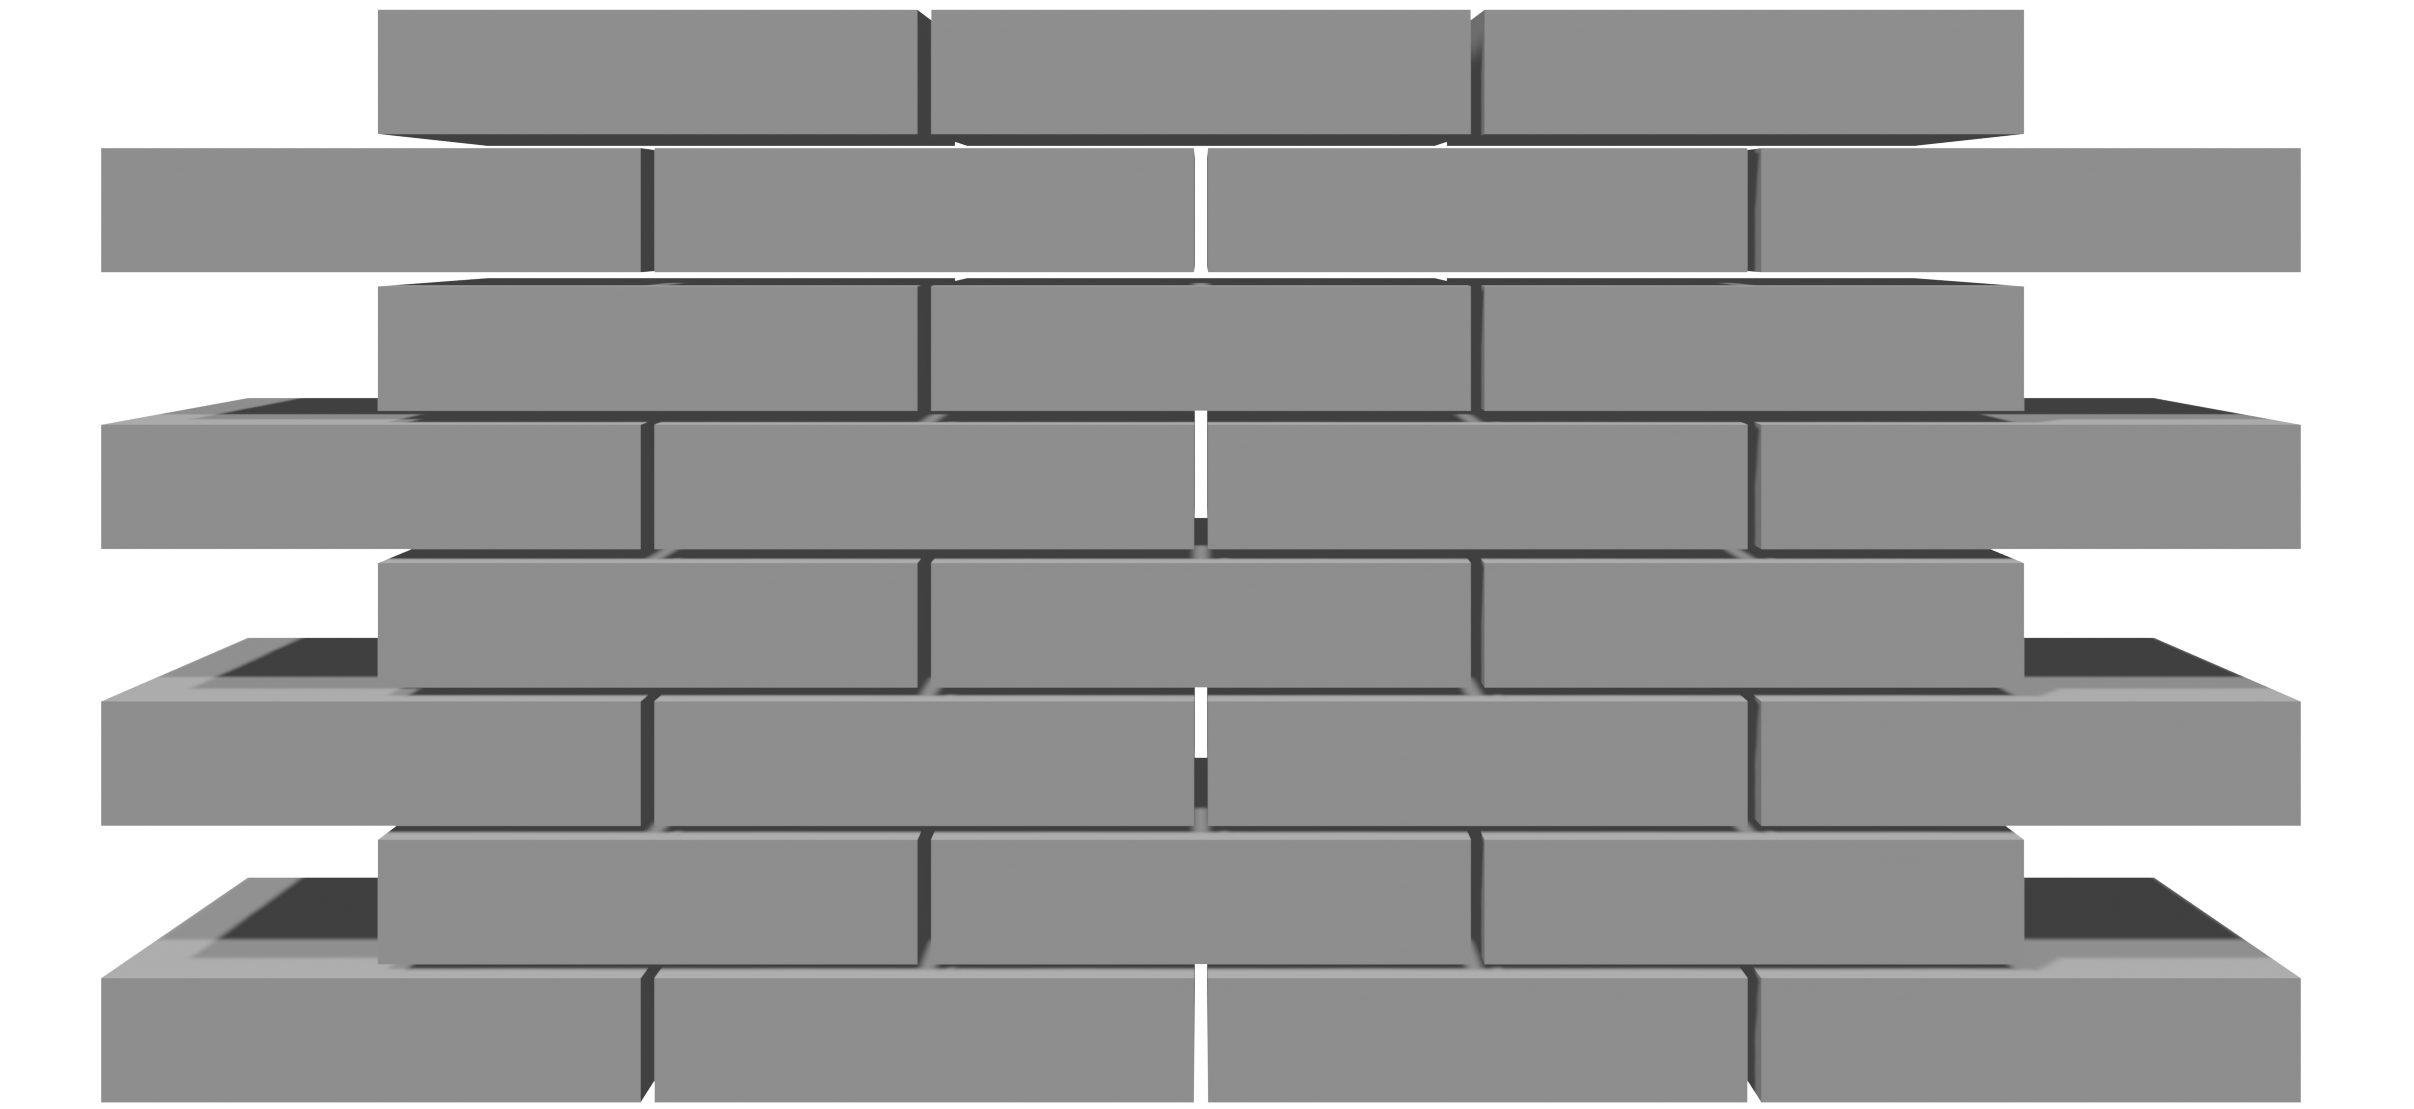
\includegraphics[width=\columnwidth]{fig/basics_stretchedbond50.png}
    \caption{Halbversetzter Läuferverband.}
  \end{subfigure}
  \hfill
  \begin{subfigure}[b]{0.4\columnwidth}
    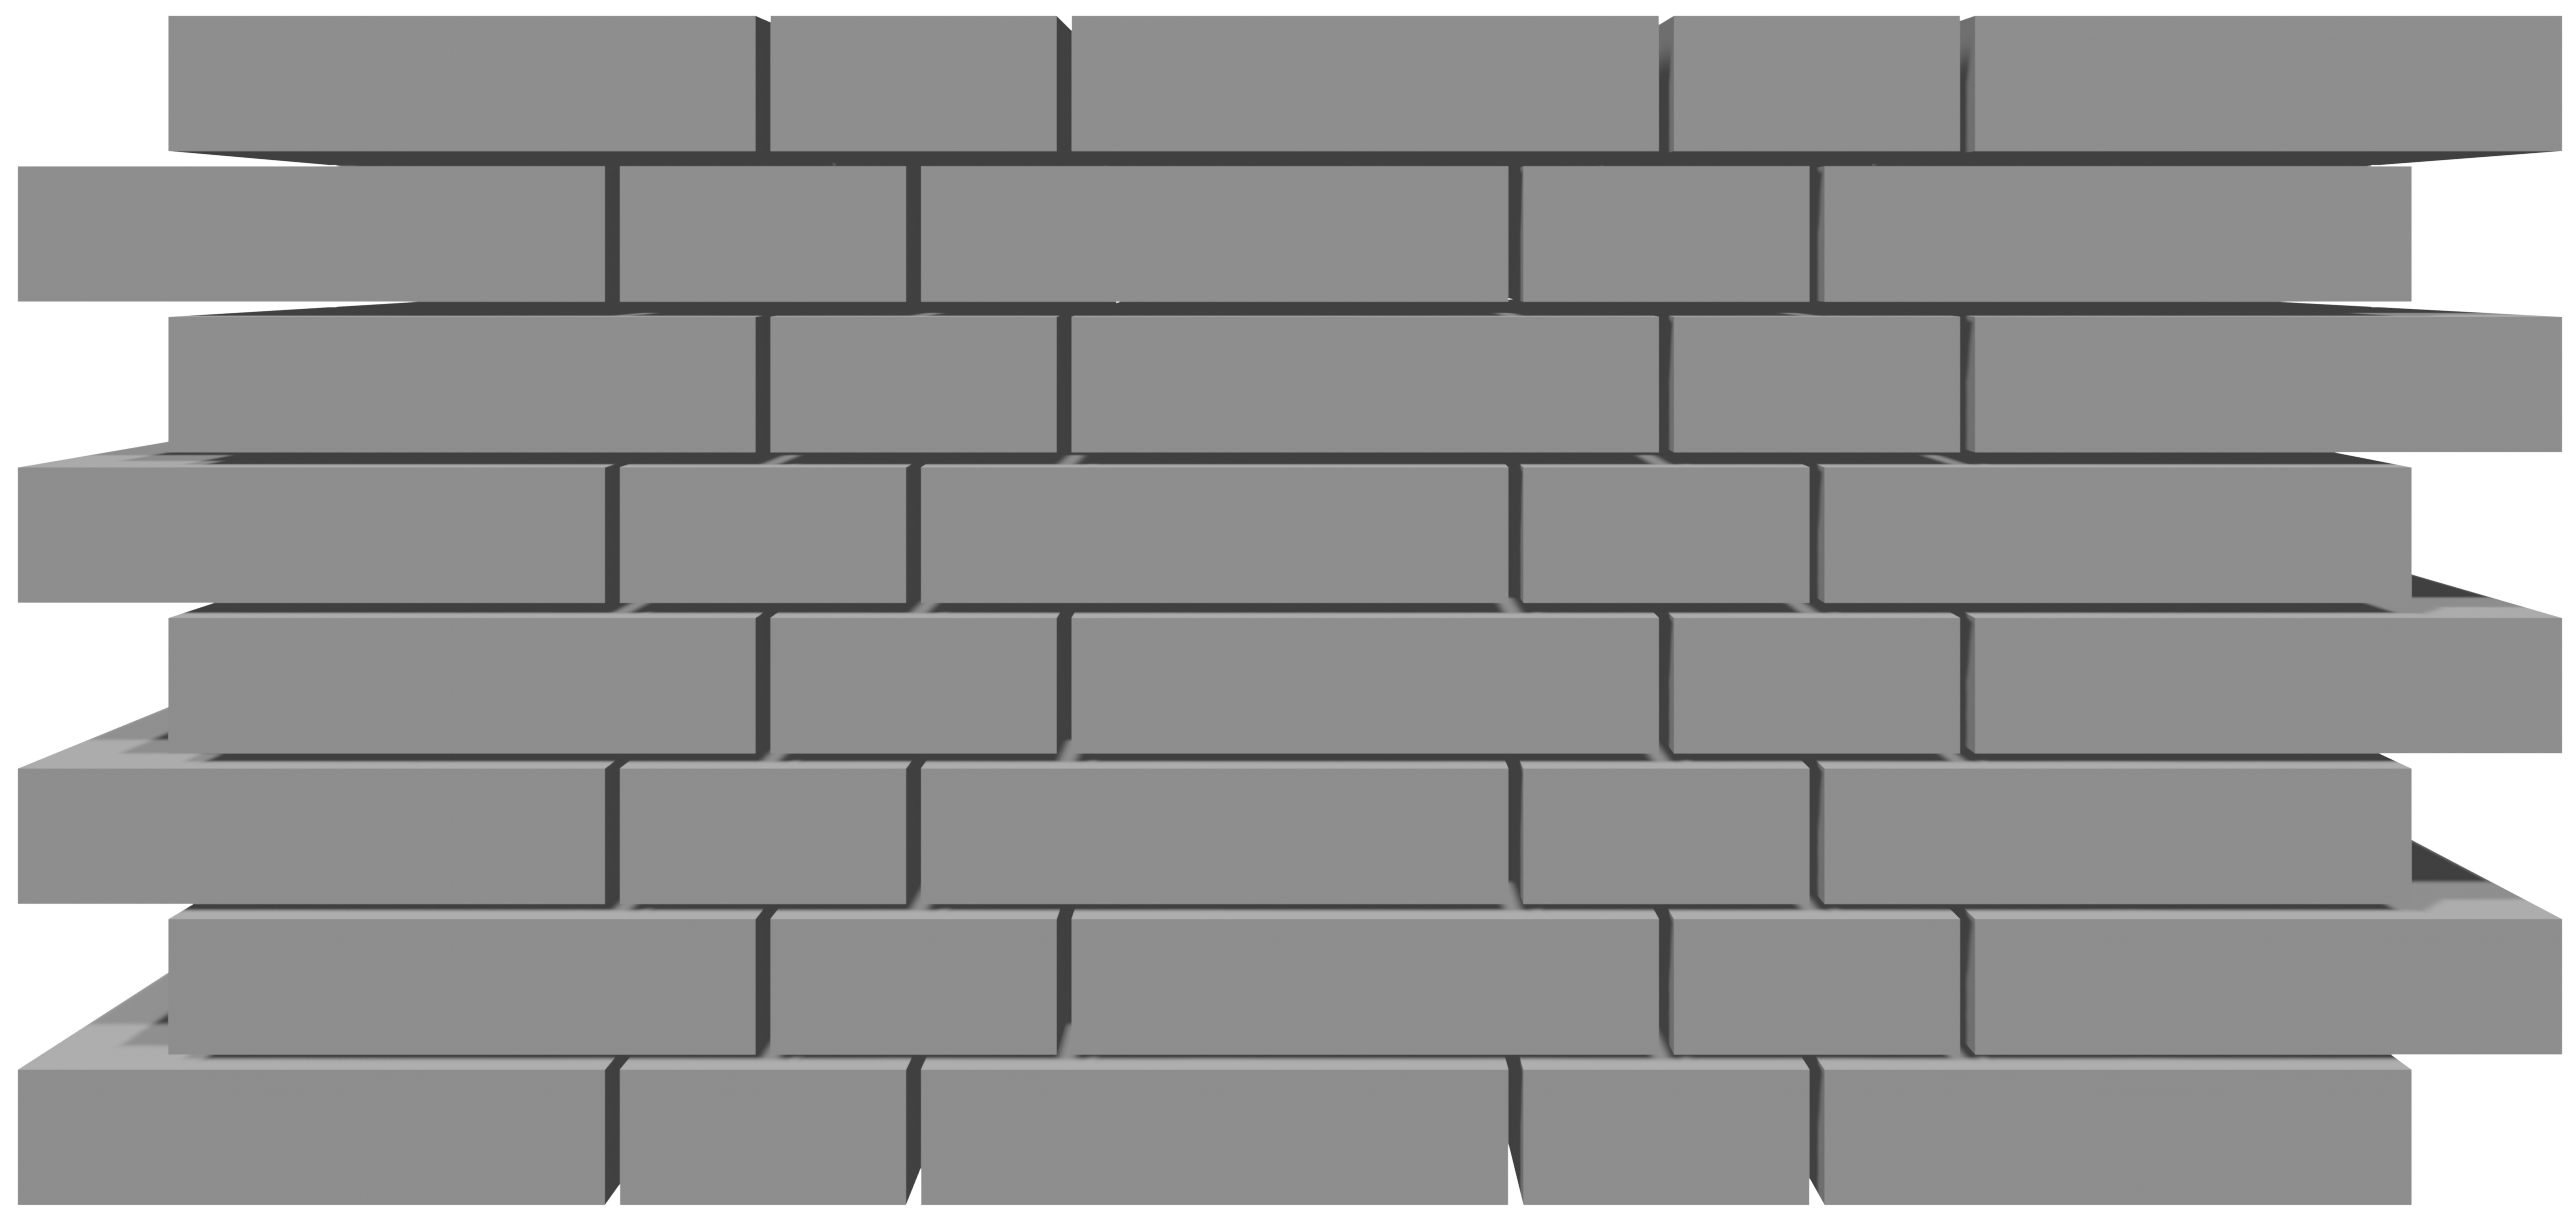
\includegraphics[width=\columnwidth]{fig/basics_gothicbond.png}
    \caption{Gotischer Verband.}
  \end{subfigure}
  \caption{Typische Mauerwerksverbände. In diesem Beispiel weisen die Läuferverbände in~\ref{fig:basics:verbaende_c} und~\ref{fig:basics:verbaende_d} einen Versatz von \(1/4\) der Steinlänge auf.}\label{fig:basics:verbaende}
\end{figure}
\subsection{Mauerwerksverband}\label{basics:Mauerwerksverband}
Als Mauerwerksverband bezeichnet man bestimmte, gleichmäßige Anordnungen von Mauersteinen, um einen homogenen Mauerwerkskörper zu erreichen~\cite{Mauerwer39:online}.
Damit kann eine gleichmäßige Kraftverteilung innerhalb der Mauer gewährleistet werden.
Eine wichtige Rolle nimmt dabei das Überbindemaß ein, welches die Mindestüberlappung von Mauersteinen aus zwei Schichten der Mauer vorgibt.
Für das planmäßige Überbindemaß \(l_{ol}\) gilt für übliche Mauersteine mit Schichthöhen 
\(h_{u} \leq 249 mm\) 
nach DIN EN 1996-1-1: 
\(l_{ol} \geq 0,4h_{u} \geq 45 mm\)
~\cite{Bemessun72:online}\cite{DIN_EN_1996_1_1}.
Zudem wird darin die Mindestwanddicke für tragendes Mauerwerk, \glqq{}sofern aus Gründen der Standsicherheit, der Bauphysik oder des Brandschutzes nicht größere Dicken erforderlich sind\grqq{}~\cite{Bemessun72:online}, auf 
\(t_{min} = 115 mm\) 
festgelegt~\cite{DIN_EN_1996_1_1}.
Dies ist, wie in Abbildung~\ref{fig:basics:Steinformate} zu sehen, exakt die Breite der kleinsten Ziegelformate NF und DF.
Man unterscheidet zwei Arten von Mauerwerk: das Einsteinmauerwerk und das Verbandsmauerwerk.
\begin{figure}[htb]
  \centering
  \includegraphics[width=0.7\columnwidth]{fig/KreuzungslösungBeispiel.png}
  \caption{Lösung einer Kreuzung am Beispiel einer \glqq{}Wand aus 2 DF im Kreuz- und Blockverband\grqq{}~\cite{MaurerfibelKreuzungen:online}.}\label{fig:basics:Kreuzungsloesung}
\end{figure}
Wie schon dem Namen zu entnehmen, handelt es sich beim Einsteinmauerwerk und ein Mauerwerk, bei welchem die Wanddicke der Steinbreite entspricht.
Hier muss das Überbindemaß lediglich über die Wandlängsrichtung eingehalten werden.
Bei Verbandsmauerwerk gilt dies zusätzlich für die Wandquerrichtung~\cite{05maurer1:online}.
Einige Beispiele sind in Abbildung~\ref{fig:basics:verbaende} zu sehen.
Als Wandstück wird von nun an ein gerader Wandabschnitt bezeichnet.
Dieser hat eine Länge, eine Höhe und durch einen vorgegebenen Bausteintyp und einem gewünschten Verband eine gewisse Breite.
Treffen zwei oder mehrere Wandstücke aufeinander, so gilt es diese dem Überbindemaß entsprechend miteinander zu verzahnen.
Dabei treten verschiedene Sonderfälle auf, die für unterschiedliche Verbände nach unterschiedlichen Lösungen verlangen:
\begin{itemize}
  \item \textbf{Ecken} werden durch zwei sich an Wandenden berührenden, meist rechtwinklig zueinanderstehenden Wandstücken gebildet.
  \item \textbf{Kreuzungen} stellen zum Beispiel zwei sich kreuzende Wandstücke dar.
  \item \textbf{T-Kreuzungen} entstehen, wenn ein Wandende des einen Wandstücks auf einer anderen Wand steht.
  Sowohl bei Kreuzungen als auch T-Kreuzungen kann auf das aufwendige Verzahnen verzichtet und stattdessen die sogenannte Stumpfstoßtechnik angewandt werden.
  Dabei werden Stahlanker zwischen der Wand und den darauf treffenden \glqq{}stumpfen\grqq{} Wandenden verwendet, um die beiden Wände sicher miteinander zu verbinden.
  \item \textbf{Wandenden} sind die \glqq{}Enden\grqq{} eines Wandstücks, die kein anderes Wandstück berühren.
  Dafür muss der verwendete Mauerwerksverband zu einem geraden Abschluss gebracht werden.
  Oftmals lässt sich das Anpassen der Bausteine (etwa durch Zerschneiden) nicht vermeiden.
  \item \textbf{Öffnungen} innerhalb eines Wandstücks können in derselben Art behandelt werden, da der vorherrschende Verband in den betroffenen Schichten gerade unterbrochen werden muss.
  Über Öffnungen für Fenster und Türen wird ein sogenannter Sturz gelegt, welcher ebenfalls in den der Wand zugrunde liegenden Mauerwerksverband eingebunden werden muss.  
\end{itemize}

\begin{figure}[ht]
  \centering
  \includegraphics[width=0.9\columnwidth]{fig/Eck- und Kreuzungslösungen.png}
  \caption{Lösungen für Ecken und T-Kreuzungen unterschiedlicher Verbände~\cite{Moro2021}.}\label{fig:basics:mauerwerk_eckloesung}
\end{figure}
Die Lösungen für die oben genannten Situationen variieren je nach angestrebten Mauerwerksverband und der verwendeten Modulgröße stark.
Einige Beispiele sind in Abbildung~\ref{fig:basics:mauerwerk_eckloesung} und Abbildung~\ref{fig:basics:Kreuzungsloesung} zu sehen~\cite{Moro2021}\cite{MaurerfibelKreuzungen:online}.
Während etwa beim Läuferverband manchmal darauf verzichtet werden kann Bausteine für Eckbereiche und Kreuzungen zu zerschneiden, ist dies für andere Verbände teilweise unumgänglich. 

\begin{figure}[hb]
  \centering
  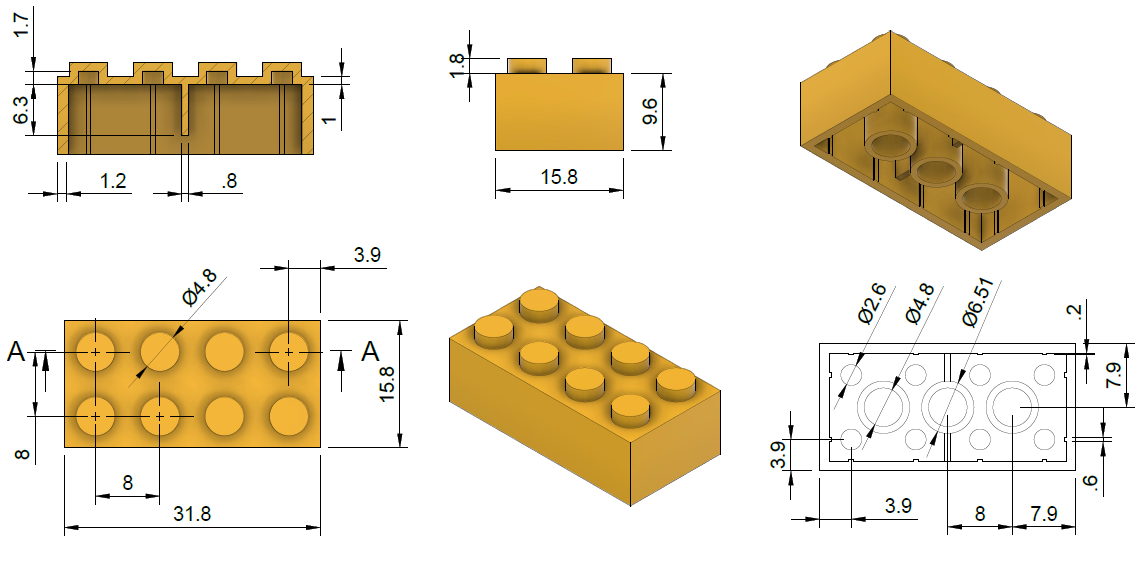
\includegraphics[width=0.85\columnwidth]{fig/LEGO 2mal4 Brick horizontal.png}
  \caption{Maße des Standard 2$\times$4 LEGO Steins~\cite{LEGOBric2:online}.}\label{fig:basics:Lego 2x4 Brick}
\end{figure}
\section{LEGO System}\label{basics:lego}
Ein 1$\times$1 LEGO Stein hat eine quadratische Grundfläche von \(7.8 mm\)$\times$\(7.8 mm\).
Dies entspricht demnach dem Baunennmaß des 1$\times$1 LEGO Steins.
Zwischen zwei nebeneinander platzierten Steinen ist ein Abstand von  \(0.2 mm\).
Daraus ergibt sich ein Baurichtmaß beziehungsweise ein Rastermaß von \(8 mm\)$\times$\(8 mm\).
In Abbildung~\ref{fig:basics:Lego 2x4 Brick} werden zur Veranschaulichung die Maße des populären 2$\times$4 Steines aufgeschlüsselt.
Die für ein dreidimensionales Maß noch fehlende Größe ist die Höhe der Steine.
Diese beträgt \(9.6 mm\).
Der Abstand zwischen zwei übereinander gestapelten Steinen hängt von dem Druck ab, der beim Zusammenstecken geleistet wurde.
Dennoch kann dieser vernachlässigt und demnach als Abstand von \(0.0 mm\) gewertet werden.

\section{Ontologie}\label{basics:ontologie}
Der Begriff Ontologie stammt ursprünglich aus der Philosophie.
Wörtlich übersetzt bedeutet er \glqq{}Lehre des Seins\grqq{}.
Ein Definitionsvorschlag lautet wie folgt (aus dem Englischen):
\glqq{}Die Ontologie als Teilgebiet der Philosophie ist die Wissenschaft von dem, was existiert, den Arten und Strukturen von Objekten, Eigenschaften, Ereignissen, Prozessen und Relationen in allen Bereichen der Wirklichkeit\grqq{}~\cite{Ontology}.
Eine Anmerkung, die oftmals im Anschluss eines Definitionsvorschlags zu finden ist, besagt, dass dabei nicht nur das, \textit{was ist}, sondern ebenfalls das, \textit{was sein könnte} betrachtet werden müsse~\cite{Ontology}\cite{OntologieDefinitionLMU:online}.
Dieser Gedanke spiegelt sich ebenfalls in dem Ontologiebegriff aus der Informatik wider und ist unter dem Begriff \textit{Open World Assumption} bekannt.
Diese Eigenschaft wird nach der Definition von Ontologien im Kontext der Informatik noch einmal ausführlicher aufgegriffen.

Im Fachbereich der Informatik wurde der Begriff Ontologie adaptiert und zunächst als \glqq{}explicit specification of a conceptualization\grqq{} definiert~\cite{Gruber1993}.
Wörtlich übersetzt lautet diese Definition etwa \glqq{}explizite Spezifizierung einer Konzeptualisierung\grqq{}.
Im Laufe der Jahre wandelte sich diese Definition, sodass sich daraus zum Beispiel folgendes ergab: \glqq{}An ontology is a formal, explicit specification of a shared conceptualization\grqq{}~\cite{Studer1998}.
Hier wird eine Ontologie also als \glqq{}formale, explizite Spezifizierung einer geteilten Konzeptualisierung\grqq{} bezeichnet.
Den wichtigsten Zusatz hierbei stellt das Wort \glqq{}geteilt\grqq{} dar, da Ontologien unter anderem dem Zweck dienen, Informationen und Vokabulare mehrerer Wissensrepräsentationen zu vereinen.
Der Begriff Konzeptualisierung wird oft als \glqq{}vereinfachte, abstrakte Sicht auf einen für einen bestimmten Nutzen relevanten Teil der Welt\grqq{} beschrieben~\cite{Guarino2009}.

Eine solche \glqq{}Spezifizierung einer Konzeptualisierung\grqq{} einer gewissen Domäne kann heutzutage mithilfe der sogenannten \textit{Web Ontology Language} (OWL), welche auf dem \textit{Resource Description Framework} (RDF) aufbaut, realisiert werden~\cite{OWL_W3C}\cite{RDF_W3C}.
OWL erlaubt es Klassen zu definieren und daran Eigenschaften anzuheften.
Außerdem können sogenannte Individuen beziehungsweise Instanzen erstellt werden.
Diese realisieren eine oder mehrere Klassen.
Mithilfe dieser Klassen, Eigenschaften und Individuen können sogenannte \textit{Reasoner} logische Schlussfolgerungen über implizit angegebenes Wissen ziehen.
Eine Ontologie kann damit einerseits etwa mit neuen Klassenzuordnungen oder implizit angegeben Vererbungen erweitert, andererseits auf Validität überprüft werden.
Werden Verletzungen von aufgestellten Axiomen oder widersprüchliche Einschränkungen von Klassen oder Eigenschaften entdeckt, so kann ein Reasoner diese nicht nur melden, sondern auch mithilfe logischer Beweisführung herleiten.
Damit stellen Reasoner ein wertvolles Werkzeug für die Entwicklung und Erweiterung von Ontologien dar.
Drei weit verbreitete Reasoner sind: 
\newpage
\begin{itemize}
  \item ELK Reasoner der Universitäten Ulm und Oxford~\cite{Kazakov2014}.
  \item HermiT Reasoner von der \textit{Information Systems Group} der Universität Oxford~\cite{Glimm2014}\cite{HermitReasoner:online}.
  \item Open Source Pellet Reasoner der Clark \& Parsia LLC~\cite{Sirin2007}. 
\end{itemize}
Aufgrund der oben genannten Idee der \textit{Open World Assumption} unterscheidet sich die Art der Reasoner logische Schlussfolgerungen zu ziehen von der, mit welcher logische Aussagen von zum Beispiel Programmiersprachen bewertet werden.
Im Grunde versteht man unter der \textit{Open World Assumption}, das nicht falsifizieren eines logischen Ausdrucks, falls Wissen existieren könnte, das den Ausdruck doch verifizieren würde.
Ein Reasoner beziehungsweise eine Programmiersprache im Kontext der \textit{Closed World Assumption} würde in so einer Situation davon ausgehen alle existierenden Informationen darüber bereits vorliegen zu haben und eventuell zu einem anderen Schluss gelangen.
Definiert man zum Beispiel eine Klasse A als alle Individuen, die nur eine Eigenschaft E besitzen, die sie mit Individuen einer bestimmten anderen Klasse B verbindet, so kann ein Reasoner innerhalb dieser Ontologie ein Individuum, das zwar diese Anforderung erfüllt, nicht der Klasse A zuordnen, da es sein kann, dass zu einem späteren Zeitpunkt (oder an anderer Stelle) Informationen existieren, die diese Zuordnung fehlerhaft machen würden.
In einer Umgebung, in der die \textit{Closed World Assumption} gilt, wäre diese Zuordnung hingegen völlig korrekt.
Die Annahme einer \textit{offenen Welt} ermöglicht es ebenfalls die Idee des sogenannten \glqq{}Semantic Web\grqq{} mithilfe von Ontologien zu realisieren~\cite{SemanticWebLee}.
Denn die Natur des Internets entspricht eher einer sich ständig ändernden und offenen Welt, als einer Geschlossenen.
Als Semantic Web wird das Annotieren von sämtlichen Webinhalten mit semantischen Informationen bezeichnet.
Damit wird das Ziel verfolgt, ein maschinenlesbares Internet zu schaffen. 

\subsection{Protégé}\label{basics:protege}
Protégé ist ein grafischer Editor zur Erstellung und Instandhaltung von Ontologien~\cite{Protege}.
Entwickelt wird das Programm an der Universität Stanford und ist als Open Source Anwendung kostenfrei nutzbar.
Die erste Version wurde bereits 1999 veröffentlicht.
Durch seine Plugin-Struktur können neben zahlreichen Erweiterungen beispielsweise auch neue Reasoner an das Programm angeschlossen werden.
Standardmäßig sind der ELK und der HermiT Reasoner integriert, aber es existieren Plugins, um auch Pellet in Protégé zu nutzen.
Das Arbeiten mit einem grafischen Editor erleichtert den Einstieg in das Thema und ermöglicht später einen besseren Überblick über oftmals umfangreiche Ontologien, als es in einem herkömmlichen Texteditor möglich wäre.
Darum wurde das Programm zur Erstellung einer Ontologie für diese Arbeit herangezogen.

\subsection{Owlready2}\label{basics:owlready}
Owlready2 ist eine Python 3 Bibliothek, die es ermöglicht \textit{ontologieorientiert} zu programmieren~\cite{Owlready}.
Bisher mussten Ontologien mithilfe von Abfragesprachen (etwa SPARQL) oder APIs bearbeitet und ausgewertet werden~\cite{SPARQLF_W3C}.
Owlready2 bietet hingegen einen einfacheren Umgang mit Ontologien, ebnet damit den Einstieg in das Thema und ermöglicht gleichzeitig die Integration von Ontologien in jedes mit Python umsetzbare Projekt.
Im Zusammenspiel mit Protégé bietet diese Bibliothek eine für Programmierer intuitive Möglichkeit, die oben genannten Werkzeuge für IFC und BIM durch Nutzung von Python 3 direkt mit der Technologie der Ontologien zu koppeln.
